\chapter{列聯表分析與二元回歸}

    截至目前為止,我們探討的假說檢定及信賴區間建構中,大多假設有興趣的結果變項為連續型變數、且(誤差)服從常態分布。常態分布假設的方便之處在於,許多形式簡單的統計量將服從已知的分布,例如標準常態分布、$t$ 分布或 $F$ 分布,而這些分布有助於後續的統計推論。然而,當結果變項為類別變項,我們就失去了常態分布的假設,因此無法直接套用前述的檢定。唯二的特例是結果變項為二元變項,且對單樣本的母體比例、或兩個獨立樣本的母體比例差值有興趣的情境。此時只要樣本數足夠大,由於樣本比例可以看作白努利變數的樣本平均,根據中央極限定理,我們可以用常態分布來近似針對母體比例或母體比例差值的檢定或信賴區間。然而,我們常想對類別變項探討更複雜的統計問題:如果類別變項有三個以上的層次,是否可以檢定三個層次的母體比例是否均等?我們可以用相關係數及線性回歸探討兩個連續變項的相關性,那麼如何檢定兩個類別變項是否彼此相關?如何以類別變項為反應變數,連續變項為解釋變數建立模型?本章我們將從列聯表分析出發,探討如何進行以類別變項為結果變項的檢定與模型建立。
    
    \begin{introduction}[第 \thechapter 章學習目標]
        \item 類別資料與列聯表的整理
        \item 四種卡方檢定:適合度檢定、同值性檢定、獨立性檢定與麥內瑪檢定
        \item 了解葉氏校正及費雪精確檢定的目的與使用時機
        \item 了解羅吉斯回歸的假設與回歸係數解釋
    \end{introduction}

\section{單因子列聯表與卡方適合度檢定}

    為了討論方便,本章我們將運用表 \ref{tab:documentary_data} 的假想資料。該資料為衛生單位在全台巡迴舉辦癌症篩檢衛教取得的問卷結果,共取得 1500 份具代表性的問卷。其中教育程度為類別變項,共有碩博士、大專、高中職、國中以下四個層次;性別為二元類別變項,層次為男或女;年齡為連續變項;衛教前和衛教後願意篩檢均為二元變項,層次為是或否。
    
    \begin{table}[htbp]
        \begin{center}
            \begin{tabular}{cccccc}
                \toprule
                問卷編號 & 居住地 & 性別 & 年齡 &  衛教前願意篩檢 & 衛教後願意篩檢\\
                \hline
                1 & 碩博士 & 男 & 40 & 是 & 是\\
                2 & 碩博士 & 女 & 26 & 否 & 是\\
                3 & 國中以下 & 男 & 30 & 是 & 否\\
                4 & 高中職 & 女 & 35 & 是 & 是\\
                5 & 大專 & 女 & 24 & 否 & 是\\
                6 & 高中職 & 女 & 17 & 否 & 是\\
                $\vdots$ & $\vdots$ & $\vdots$ & $\vdots$ & $\vdots$ & $\vdots$ \\
                \bottomrule
            \end{tabular}
            \caption{癌症篩檢衛教的調查資料\label{tab:documentary_data}}
        \end{center}
    \end{table}

    假設我們對各教育程度的比例有興趣。我們在敘述統計的部分有討論到,頻率表可以描述類別變項完整的分布資訊,因此可以我們可以先做出如表 \ref{tab:one_way_contingency} 上方的頻率表。頻率表又被稱為 \textit{單因子列聯表} (one-way contingency table),其中稱為\textit{列聯表} (contingency table) 的原因是因為它以矩陣形式記錄了資料中各種子族群的人數,而單因子則表示子族群僅由單一個類別變項作分類。現在我們已知教育部統計的全國教育程度比例為碩博士 $8.6\%$、大專 $41.6\%$、高中職 $28.8\%$、國中以下 $21.0\%$,並想要檢定接受衛教族群的教育程度分布是否符合全國教育程度比例。換言之,我們的虛無假說和對立假說分別為:
    \[\left\{\begin{array}{l}
        H_0: \text{表\ref{tab:one_way_contingency}上表各格的母體比例分別為($8.6\%$, $41.6\%$, $28.8\%$, $21.0\%$)}\\
        H_1: \text{表\ref{tab:one_way_contingency}上表各格的母體比例並非上述分布}
    \end{array} \right.\]
    這種檢定的目的是想了解資料是否符合虛無假說預想的分布,因此也被稱為\textit{適合度檢定} (goodness-of-fit test)。
    
    \begin{table}[htbp]
        \begin{center}
            \begin{tabular}{cccc|c}
                \toprule
                碩博士 & 大專 & 高中職 & 國中以下 & 總和\\
                \hline
                138 & 634 & 459 & 269 & 1500\\
                \bottomrule
            \end{tabular}
            
            \bigskip
            
            \begin{tabular}{c|cccc|c}
                \toprule
                 & 碩博士 & 大專 & 高中職 & 國中以下 & 總和\\
                \hline
                觀察值 & 138 ($O_1$) & 634 ($O_2$) & 459 ($O_3$) & 269 ($O_4$) & 1500\\
                預期值 & 129 ($E_1$) & 624 ($E_2$) & 432 ($E_3$) & 315 ($E_4$) & 1500\\
                \bottomrule
            \end{tabular}
            \caption{教育程度的單因子列聯表\label{tab:one_way_contingency}}
        \end{center}
    \end{table}

    為了建構上述適合度檢定所需的檢定統計量,我們可以先試算,如果這 $1500$ 份問卷中,教育程度分布真的符合 ($8.6\%$, $41.6\%$, $28.8\%$, $21.0\%$),那麼我們預期每一種教育程度的人數應該是多少。計算方式非常簡單,只要把人數乘上機率即可,例如碩博士的預期人數為 $1500 \times 8.6\% = 129$ 人、大專的預期人數為 $1500 \times 41.6\% = 624$ 人…等等。將預期人數與實際觀察到的人數並列即如表 \ref{tab:one_way_contingency} 下方的表格所示,其中為了符號化方便,我們以 $O_1$ 到 $O_4$ 代表四組的觀察值 (\textbf{o}bserved value),而以 $E_1$ 到 $E_4$ 代表四組的預期值 (\textbf{e}xpected value)。直覺上,如果觀察值離預期值越遠,代表資料越偏離虛無假說下的比例。因此,根據我們上一章最小平方法的想法,如果要建構檢定統計量,應該可以將觀察值和預期值差值的平方加總,總和值若很大則暗示觀察值偏離預期值,因此虛無假說不成立:
    \[\sum_{i=1}^4 (O_i - E_i)^2 = (138-129)^2 + (634-624)^2 + (459-432)^2 + (269-315)^2\]
    注意到,上述的計算方法將每一格的重要性視為相同。也就是說,「在碩博士這組的觀察預期人數差值為 10」和「在大專這組的觀察預期人數差值為 10」對於平方和的貢獻程度相同。然而在列聯表中,每一格觀察值的變異性會和其預期值有關。同樣是觀察預期人數差值為 10,如果該格的變異性本來就較大,那麼這個差值可能只是因為抽樣造成的隨機變異;相反的,如果該格的變異性很小,那麼這個差值就很可能代表資料偏離了預期比例。根據上述的思路,Karl Pearson 於 1900 年提出應該\textbf{用各個格子的期望值來標準化平方和},也就是:
    \[X^2 = \sum_{i=1}^4 \frac{(O_i - E_i)^2}{E_i} = \frac{(138-129)^2}{129} + \frac{(634-624)^2}{624} + \frac{(459-432)^2}{432} + \frac{(269-315)^2}{315} \approx 9.193\]
    在虛無假設下,隨著樣本數增加使得每個格子的期望值「夠大」,Karl Pearson 證明上述檢定統計量的虛無分布近似於\textit{卡方分配} (chi-squared distribution),因此該檢定統計量被稱為\textit{卡方統計量} (chi-squared statistic)、檢定又名\textbf{卡方適合度檢定}。卡方分配是一個取值恆正、右偏的連續分配,且有一個稱為\textit{自由度} (degrees of freedom) 的參數,其機率密度函數如圖 \ref{fig:chi_squared} 所示。在卡方檢定中,卡方統計量虛無分配的自由度為在虛無假說下「列聯表中能夠自由變動的觀察值數目」減去「計算期望值時利用觀察值估計的參數個數」。在表\ref{tab:one_way_contingency} 中,觀察值雖然有 $138$、$634$、$459$ 和 $269$ 四個,但它們加起來必須是樣本數 $1500$,因此實際上只有三個觀察值能自由變動;而在計算期望值時,我們完全沒有用到觀察值的資訊,估計的參數個數為零;因此,該卡方檢定量的虛無分布應為自由度等於 $3$ 的卡方分布。一般性地來說,如果類別變項有 $k$ 個層次,且欲檢定各層次的母體比例是否和已知的比例相符,則卡方適合度檢定的統計量及虛無分布可寫為:
    \[X^2 = \sum_{i=1}^k \frac{(O_i - E_i)^2}{E_i} \xrightarrow[]{d} \chi^2_{k-1}\]

    \begin{figure}[htbp]
        \centering
        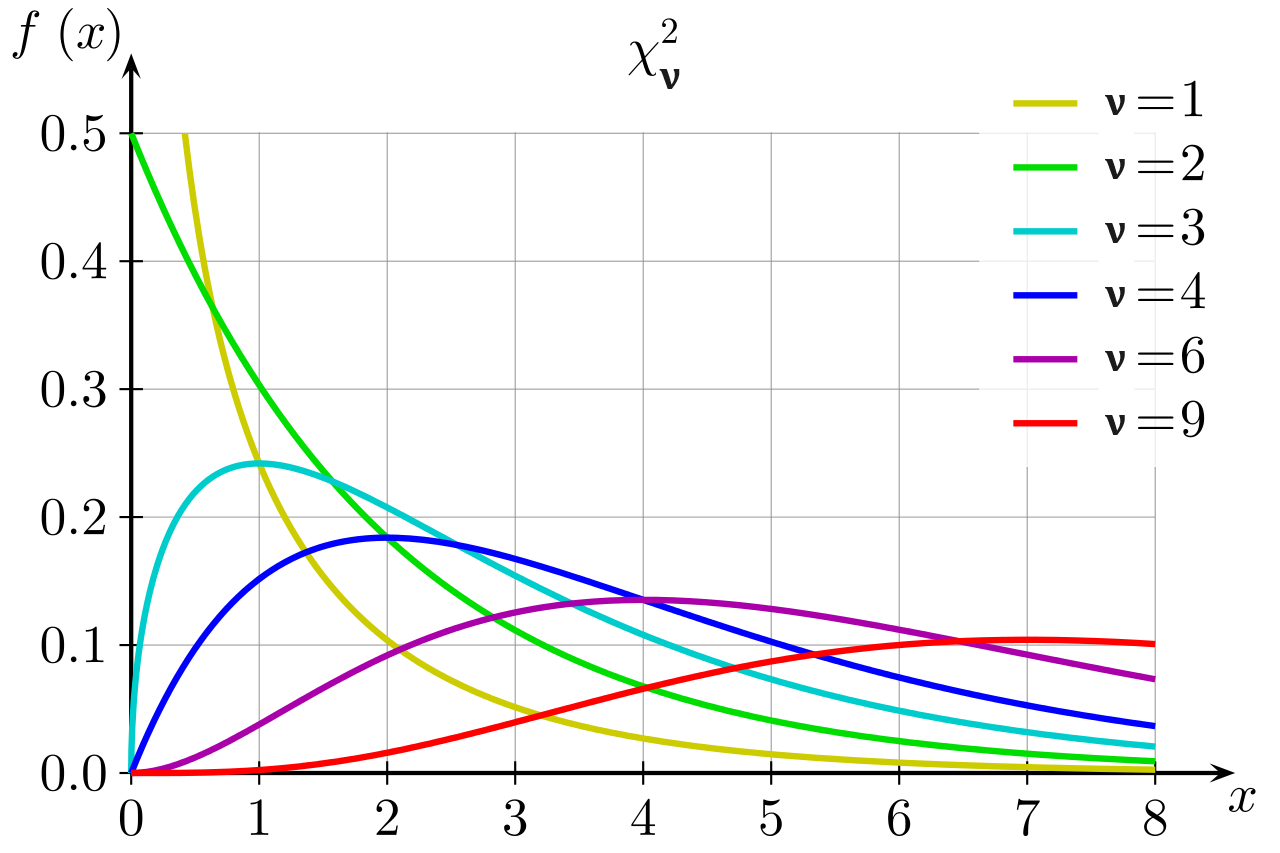
\includegraphics[width=0.5\textwidth]{figures/09-Contingency_table_binary_regression/Chi_square.png}
        \caption{卡方分配的機率密度函數,$\nu$ 代表卡方分配的自由度}
        \label{fig:chi_squared}
    \end{figure}

    由於卡方統計量取值越大,代表觀察值越偏離期望值,亦即資料越偏向對立假說,因此卡方適合度檢定的 $p$ 值應該取卡方分布右邊尾巴的機率,也就是 $\PP(\chi^2_{k-1} \ge X^2)$。同樣地,如果要用拒絕域法進行檢定,則拒絕域也會是右尾,因此在顯著水準為 $\alpha$ 的情況下,拒絕區為 $X^2 \ge \chi^2_{k-1, \alpha}$,其中 $\chi^2_{k-1, \alpha}$ 為 $\chi^2_{k-1}$ 右尾機率為 $\alpha$ 的臨界值。

    在上述的例子中,卡方統計量的取值為 $9.193$。計算 $p$ 值得到 $\PP(\chi^2_3 \ge 9.193) \approx 0.027$;另外,在顯著水準定為 $0.05$ 下,卡方統計量的拒絕域為 $X^2 \ge \chi^2_{3,0.05} \approx 7.81$。兩種方法都顯示,在顯著水準為 $0.05$ 下拒絕虛無假說,也就是這份問卷背後的母體族群教育程度分布顯著地異於全國教育程度之比例。

    \bigskip

    \begin{custom}{思考}
        當組數只有兩組時,若兩組人數觀察值分別為 $O_1$ 和 $O_2$,且我們想檢定第一組的母體比例是否為 $p_0$,此時適合度檢定的卡方檢定統計量為何?該檢定統計量和前面章節提到的單樣本比例檢定 $Z$ 統計量之間有什麼關係?
    \end{custom}
    
\section{雙因子列聯表、卡方同質性檢定與卡方獨立性檢定}

    在類別變項作為結果變項的分析中,我們也常想了解兩個類別變項之間是否有關係。此時我們可以將這兩個類別變項各種層次組合的發生次數紀錄於\textit{雙因子列聯表} (two-way contingency table) 中,例如表 \ref{tab:two_way_contingency_obs} 為我們的範例資料中「教育程度」與「衛教前願意篩檢」兩個類別變項的雙因子列聯表。為了後續符號化方便,我們把列聯表的row 數記為$r$、column 數記為 $c$、第 $i$ 個 row 第 $j$ 個 column 的觀察值記 $O_{ij}$、第 $i$ 個 row 的樣本數記為 $n_{i.}$、第 $j$ 個 column 的樣本數記為 $n_{.j}$、總樣本數記為 $n$。

    \begin{table}[htbp]
        \begin{center}
            \begin{tabular}{c|cccc|c}
                \toprule
                觀察值 & 碩博士 & 大專 & 高中職 & 國中以下 & 總和\\
                \hline
                衛教前願意篩檢 & 88 ($O_{11}$) & 402 ($O_{12}$) & 252 ($O_{13}$) & 162 ($O_{14}$) & 904 ($n_{1.}$)\\
                衛教前不願篩檢 & 50 ($O_{21}$) & 232 ($O_{22}$) & 207 ($O_{23}$) & 107 ($O_{24}$) & 596 ($n_{2.}$)\\
                \hline
                總和 & 138 ($n_{.1}$) & 634 ($n_{.2}$) & 459 ($n_{.3}$) & 269 ($n_{.3}$) & 1500 ($n$)\\
                \bottomrule
            \end{tabular}
            \caption{教育程度與衛教前篩檢意願的觀察值雙因子列聯表\label{tab:two_way_contingency_obs}}
        \end{center}
    \end{table}
    此時針對這兩個類別變項,我們有兩種可能的資料生成方式,與相對應的檢定:
    \begin{enumerate}
        \item 資料抽樣前其中一個變項各層次的觀察值數目已經固定。例如我們對六都居民的教育程度分佈差異有興趣,因此從台北市、新北市、桃園市、台中市、台南市、高雄市各隨機抽取了 300 位市民並調查每位市民的教育程度。此時如果針對「直轄市別」和「教育程度」作列聯表,則各個直轄市的總人數在抽樣前即已知而沒有變異性。這種情境下我們有興趣的問題是,各直轄市的教育程度分布是否不同。換句話說,我們想知道教育程度的分布在各直轄市之間是否\textit{同質} (homogeneity)。這類檢定被稱為 \textit{同質性檢定} (Test of homogeneity)。
        \item 兩個變項均為隨機抽樣。例如表 \ref{tab:two_way_contingency_obs} 中,我們在取得資料時並未對問卷填答者的衛教前篩檢意願及教育程度做任何篩選。這種情境下我們有興趣的問題是,「衛教前篩檢意願」和「教育程度」這兩個變項在資料中是否獨立。這類檢定被稱為 \textit{獨立性檢定} (Test of independence)。
    \end{enumerate}
    雖然上述兩種檢定在概念上略有不同,但實際進行檢定時,檢定統計量的計算方法與其虛無分佈均相同,因此這裡我們只針對獨立性檢定進行後續探討。獨立性檢定的虛無假說及對立假說分別為:
    \[\left\{\begin{array}{l}
        H_0: \text{表\ref{tab:two_way_contingency_obs}中每位填答者的衛教前篩檢意願和其教育程度獨立}\\
        H_1: \text{表\ref{tab:two_way_contingency_obs}中每位填答者的衛教前篩檢意願和其教育程度不獨立}
    \end{array} \right.\]
    而後我們參考配適度檢定的流程,試著算出虛無假說下每個格子的人數期望值。由於在虛無假說下篩檢意願和教育程度獨立,根據獨立的定義,資料中「碩博士且願意篩檢」的母體比例應等於「碩博士」的母體比例乘上「願意篩檢」的母體比例。然而此處我們不知道後面兩個母體比例,只能用資料下去估計:碩博士共有 $n_{.1} = 138$ 位,因此估計佔總體比例為 $n_{.1}/n = 138/1500$;願意篩檢者共有 $n_{1.} = 904$ 位,因此估計佔總體比例為 $n_{1.}/n = 904/1500$。因此,虛無假設下「碩博士且願意篩檢」的母體比例估計值為兩者相乘:$(n_{1.}/n)(n_{.1}/n) = (138/1500)(904/1500)$。最後,總樣本數乘上比例估計值即為「碩博士且願意篩檢」的人數期望值(我們記為 $E_{11}$):
    \[E_{11} = n \cdot \frac{n_{1.}}{n} \cdot \frac{n_{.1}}{n} = \frac{n_{1.}n_{.1}}{n} = \frac{904 \cdot 138}{1500} \approx 83.17\]
    同理,第 $i$ 個 row 第 $j$ 個 column 的人數期望值(記為 $E_{ij}$)可一般性地寫為該 row 樣本數($n_{i.}$)乘上該 column 樣本數($n_{.j}$)除以總樣本數:
    \[E_{ij} = \frac{n_{i.}n_{.j}}{n}\]
    將所有格子的期望值算出來後可以得到表\ref{tab:two_way_contingency_exp}。
    \begin{table}[htbp]
        \begin{center}
            \begin{tabular}{c|cccc|c}
                \toprule
                期望值 & 碩博士 & 大專 & 高中職 & 國中以下 & 總和\\
                \hline
                衛教前願意篩檢 & 83.17 ($E_{11}$) & 382.09 ($E_{12}$) & 276.62 ($E_{13}$) & 162.12 ($E_{14}$) & 904\\
                衛教前不願篩檢 & 54.83 ($E_{21}$) & 251.91 ($E_{22}$) & 182.38 ($E_{23}$) & 106.88 ($E_{24}$) & 596\\
                \hline
                總和 & 138 & 634 & 459 & 269 & 1500\\
                \bottomrule
            \end{tabular}
            \caption{教育程度與衛教前篩檢意願的期望值雙因子列聯表\label{tab:two_way_contingency_exp}}
        \end{center}
    \end{table}

    而後,我們參考適合度檢定的方法,將每個格子觀察值和期望值的差值平方,並以期望值標準化後加總,以建立卡方檢定統計量。差別只在於適合度檢定只有一個 row,而這裡我們有一整個矩陣要加總:
    \[X^2 = \sum_{i=1}^r \sum_{j=1}^c \frac{(O_{ij}-E_{ij})^2}{E_{ij}} = \frac{(88-83.17)^2}{83.17} + \frac{(402-382.09)^2}{382.09} + \cdots + \frac{(107-106.88)^2}{106.88} \approx 8.83\]
    在虛無假說下,當樣本數增加使得每個格子的期望值「夠大」時,$X^2$ 統計量的抽樣分布同樣會近似於卡方分布。我們可以思考一下該分布的自由度應該如何計算:首先我們總共有 $rc$ 個觀察值,但它們加總必須等於固定的總樣本數 $n$,因此總共有 $rc - 1$ 個可以自由變動的觀察值。但注意到我們在計算期望值時,用資料估計了兩個類別變項各階層的母體比例。在 row 代表的類別變項需要估計 $r-1$ 個母體比例(最後一個層次的比例用 $1$ 減去其他層次的比例即可),在 column 代表的類別變項則需要估計 $c-1$ 個母體比例。因此,卡方檢定量的虛無分佈自由度為「可以自由變動的觀察值數目」減去「用資料估計的參數個數」,即$(rc-1) - [(r-1) + (c-1)] = (r-1)(c-1)$。因此,一般性地來說,檢定兩個各有 $r$ 和 $c$ 個層次的類別變項是否獨立時,卡方獨立性檢定的統計量及虛無分布可寫為:
    \[X^2 = \sum_{i=1}^r \sum_{j=1}^c \frac{(O_{ij}-E_{ij})^2}{E_{ij}} \xrightarrow[]{d} \chi^2_{(r-1)(c-1)}\]

    和適合度檢定同理,卡方統計量取值越大,資料越偏向對立假說,因此卡方獨立性檢定的 $p$ 值也應該取右尾機率,也就是 $\PP(\chi^2_{(r-1)(c-1)} \ge X^2)$。如果用拒絕域法進行檢定,則拒絕域也會是右尾,因此在顯著水準為 $\alpha$ 的情況下,拒絕區為 $X^2 \ge \chi^2_{(r-1)(c-1), \alpha}$。在上述的例子中,卡方統計量的取值為 $8.83$,且其虛無分布近似於自由度等於 $(4-1)(2-1) = 3$ 的卡方分布。計算 $p$ 值得到 $\PP(\chi^2_3 \ge 8.83) \approx 0.032$;另外,在顯著水準定為 $0.05$ 下,卡方統計量的拒絕域為 $X^2 \ge \chi^2_{3,0.05} \approx 7.81$。兩種方法都顯示,在顯著水準為 $0.05$ 下拒絕虛無假說,也就是參加衛教的群體中,衛教前篩檢的意願和教育程度有顯著相關。

    卡方獨立性(同質性)檢定統計量之虛無分佈雖然可近似為 $\chi^2_{(r-1)(c-1)}$,但在兩個情境下該近似的效果較差:第一是當列聯表為 $2 \times 2$ 時,第二是當樣本數不夠多,以至於有格子的期望值在 $5$ 以下時。當列聯表為 $2 \times 2$ 時,可以考慮使用統計學家 Frank Yates (1902-1994) 提出的\textit{葉氏連續性校正} (Yates' continuity correction),將卡方統計量修改如下:
    \[X^2 = \sum_{i=1}^2 \sum_{j=1}^2 \frac{\max(|O_{ij}-E_{ij}|-0.5)^2,0)}{E_{ij}}\]
    可以看出,分子的部分當觀察值等於期望值時仍取值 $0$,當觀察值不等於期望值時則將差異往 $0$ 靠近 $0.5$ 後再平方。因此,葉氏連續性校正會讓卡方統計量變小,使檢定變得不容易顯著,以保持可接受的型一錯誤率。當有格子的期望值在 $5$ 以下時,則建議不再使用依賴於近似的卡方檢定,並改用\textit{費雪精確檢定} (Fisher's exact test)。費雪精確檢定是用資料的精確分佈來進行檢定,並不牽涉到近似,但其計算較複雜。幸運地是,當今的統計軟體均有提供費雪精確檢定,而且不需太多耗時即可完成計算。(事實上,依現在的電腦計算能力,任何獨立性或同質性檢定均可使用費雪精確檢定,不須限縮在格子的期望值於 $5$ 以下的情境。只是習慣上,當今研究還是在能用卡方檢定時就用卡方檢定。)費雪精確檢定的假說和結論解釋方法和卡方檢定相同,當$p$值在顯著水準以下時,代表拒絕「兩個類別變項之間獨立」的假說。
    
\section{成對類別資料與麥內瑪檢定}

    在表 \ref{tab:documentary_data} 的資料中,假設我們想知道衛教是否會影響參與者的篩檢意願。由於資料中沒有「衛教」這個變數,直覺上我們似乎可以把衛教前和衛教後的兩個變數轉置成如表 \ref{tab:dependent_data} 所示。如此我們便有兩個類別變項:衛教前後以及篩檢意願,如果這兩個二元變數不獨立,就代表衛教的確會影響篩檢意願。

    \begin{table}[htbp]
        \begin{center}
            \begin{tabular}{ccc}
                \toprule
                問卷編號 & 衛教前後 & 願意篩檢\\
                \hline
                1 & 前 & 是\\
                1 & 後 & 是\\
                2 & 前 & 否\\
                2 & 後 & 是\\
                3 & 前 & 是\\
                3 & 後 & 否\\
                4 & 前 & 是\\
                4 & 後 & 是\\
                5 & 前 & 否\\
                5 & 後 & 是\\
                6 & 前 & 否\\
                6 & 後 & 是\\
                $\vdots$ & $\vdots$ & $\vdots$\\
                \bottomrule
            \end{tabular}
            \caption{資料轉置後衛教前後和篩檢意願之資料表\label{tab:dependent_data}}
        \end{center}
    \end{table}

    為了進行卡方獨立性檢定,既定流程是將表 \ref{tab:dependent_data} 製作成雙因子列聯表並得到表 \ref{tab:mcnemar_table} 左側的表格。不過注意到,雖然我們的總樣本數只有 1500,但表 \ref{tab:mcnemar_table} 左側的總樣本數竟然有 3000!這是因為同一個人會貢獻兩筆資料,一筆是衛教前的篩檢意願、一筆是衛教後的篩檢意願,造成列聯表中四格的數字有隱含的相關性,因而違反了卡方獨立性檢定的基本假設。

    \begin{table}[htbp]
        \begin{center}
            \begin{tabular}{c|ccccc|cc}
                \cline{1-3}\cline{6-8}
                 & 願意篩檢 & 不願篩檢 &&& & 衛教後願意 & 衛教後不願意\\
                \cline{1-3}\cline{6-8}
                衛教前 & 1000 & 500 &&& 衛教前願意& 800 ($a$) & 200 ($b$)\\
                衛教後 & 1150 & 350 &&& 衛教前不願意& 350 ($c$) & 150 ($d$)\\
                \cline{1-3}\cline{6-8}
            \end{tabular}
            \caption{相依類別資料的列聯表\label{tab:mcnemar_table}}
        \end{center}
    \end{table}

    針對這個檢定問題,應該建立的列聯表如表 \ref{tab:mcnemar_table} 的右側所示,如此每位填答者僅會落在四個格子中的其中一格,因而消除了資料相依性的疑慮。在這裡我們看到,有 800 位填答者在衛教前後均願意接受篩檢、而有 150 位填答者則在衛教前後均不願接受篩檢。衛教對於這些人的意願均沒有影響,因此衛教若要能夠影響總體篩檢意願,必定來自於 (衛教前不願意, 衛教後願意) 與 (衛教前願意, 衛教後不願意) 這兩個格子。當前者的人數大於後者,則衛教後整體意願會提升;反之若前者的人數小於後者,則衛教後整體意願會下降。因此,我們可以只關注這兩個格子共 550 人,並將檢定問題轉化為:(衛教前不願意, 衛教後願意) 與 (衛教前願意, 衛教後不願意) 在這 550 人的母體比例是否相等?聰明的讀者可以發現,本檢定等價於預設兩組母體比例均為 0.5 的適合度檢定,因此其檢定統計量及虛無分布可寫為:
    \[X^2 = \frac{[b-(b+c)/2]^2}{(b+c)/2} + \frac{[c-(b+c)/2]^2}{(b+c)/2} = \frac{(b-c)^2}{b+c} \xrightarrow[]{d} \chi^2_1\]
    有些統計學家則建議此處亦使用葉氏連續性校正:
    \[X^2_{\text(Yates)} = \frac{[|b-(b+c)/2|-0.5]^2}{(b+c)/2} + \frac{[|c-(b+c)/2|-0.5]^2}{(b+c)/2} = \frac{(|b-c|-1)^2}{b+c} \xrightarrow[]{d} \chi^2_1\]
    $p$ 值與拒絕域的計算和適合度檢定相同:$p$ 值為 $\PP(\chi^2_1 \ge X^2)$,顯著水準為 $\alpha$ 的拒絕域則為 $X^2 \ge \chi^2_{1, \alpha}$。檢定結果拒絕虛無假說時,代表兩個變數之間的相關性顯著。此檢定由心理計量學家 Quinn McNemar (1900-1986) 所提出,因此被稱為\textit{麥內瑪檢定} (McNemar's test)。在我們的例子中,未使用葉氏連續性校正的卡方統計量為$(350-200)^2/(350+200) \approx 40.91$,而使用葉氏連續性校正的卡方統計量為$(|350-200|-1)^2/(350+200) \approx 40.37$,在顯著水準設定為 $0.05$下,兩者都遠超過拒絕域的臨界值 $\chi^2_{1,0.05} \approx 3.84$,代表拒絕虛無假說,衛教的確會顯著影響篩檢意願。而且,因為由不願意轉為願意的人比由願意轉為不願意的人多,所以衛教是顯著增加了篩檢意願。

\section{列聯表的變數相關性度量}
    我們現在知道如何用卡方檢定(以及麥內瑪檢定)來檢定兩個類別變數間的相關性。然而,檢定結果只能告訴我們兩者是否有顯著相關,而不能幫助我們評估相關性的強弱。讀者可能還記得,先前我們在探討兩個連續變數的相關性時,使用了皮爾森相關係數來量化相關性的強弱。然而,皮爾森相關係數運用在兩個類別變數時,有一個致命的缺點:在邊際機率 (marginal probability) 固定的強況下,皮爾森相關係數的取值範圍不再是 $-1$ 到 $1$。
    
    舉例而言,如表 \ref{tab:odds_ratio} 所示,左邊的表是觀察兩個二元變數 $X_1$ 和 $X_2$ 得到的結果,依照皮爾森相關係數的公式可以得到 $r=0.433$。這個數值看起來離 $1$ 還有點距離,因此 $X_1$ 和 $X_2$ 應該只有中度的相關性。但是我們可以思考:如果我們在收取資料前已知 $X_1$ 取值為 $1$ 的比例(又稱為 $X_1=1$ 的邊際機率)為 $\frac{100}{150}$、$X_2 = 1$ 取值為 $1$ 的比例(又稱為 $X_2=1$ 的邊際機率)為 $\frac{60}{150}$,那麼最終資料的皮爾森相關係數最大值會是多少?此時可以想像,為了要讓皮爾森相關係數最大化,我們希望 $(X_1, Y_1) = (1,1)$ 和 $(X_1, Y_1) = (0,0)$ 的人越多越好。因此,在維持各個 row 和 column 的總和不變的情況下,最大化皮爾森相關係數的資料應該形如表 \ref{tab:odds_ratio} 的右方所示,計算出的相關係數上限僅為 $r=0.577$。因此,我們觀察到的 $r=0.433$ 其實已經非常靠近上限。$X_1$ 和 $X_2$ 之間的相關性應當頗強,但是單看皮爾森相關係數的數值會讓我們誤認為它們之間僅有中度相關性。

    \bigskip

    \begin{table}[htbp]
        \begin{center}
            \begin{tabular}{c|cc|cccc|cc|c}
                \cline{1-4}\cline{7-10}
                觀察值 & $X_2=1$ & $X_2=0$ & 總和 &&& 極端值 & $X_2=1$ & $X_2=0$ & 總和\\
                \cline{1-4}\cline{7-10}
                $X_1=1$ & $55~(a)$ & $45~(b)$ & $100$ &&& $X_1=1$ & $60$ & $40$ & $100$\\
                $X_1=0$ & $5~(c)$ & $45~(d)$ & $50$ &&& $X_1=0$ & $0$ & $50$ & $50$\\
                \cline{1-4}\cline{7-10}
                總和 & $60$ & $90$ & $150$ &&& 總和 & $60$ & $90$ & $150$\\
                \cline{1-4}\cline{7-10}
            \end{tabular}
            \caption{$2 \times 2$列聯表以及皮爾森相關係數的上界\label{tab:odds_ratio}}
        \end{center}
    \end{table}

    為了對類別變數的相關性強度作更精緻、具有解釋意義的評估,流行病學家通常會用三種不同的效果度量 (effect measure):\textit{風險差} (risk difference)、\textit{風險比} (risk ratio)和\textit{勝算比} (odds ratio)。
    \begin{itemize}
        \item \textbf{風險差}:顧名思義為兩組\textit{風險} (risk)的差,即兩組事件發生機率的差。根據表\ref{tab:odds_ratio}的左側表格,如果我們有興趣的 outcome 是 $X_2$,其中 $X_2 = 1$ 代表發生事件,那麼$X_1 = 1$ 這組的風險是 $\frac{a}{a+b}$,$X_1 = 0$ 這組的風險則是 $\frac{c}{c+d}$。因此,兩組的風險差為 
        \[RD = \frac{a}{a+b}-\frac{c}{c+d}\]
        風險差大於 $0$ 代表 $X_1 = 1$ 這組的風險較高,反之亦然。風險差等於 $0$ 代表兩組的風險相等,換言之就是資料中 $X_1$ 和 $X_2$ 沒有相關。
        \item \textbf{風險比}:顧名思義為兩組風險的比值。由於歷史原因,風險比 (risk ratio) 也被稱為 \textit{相對風險} (relative risk),不過兩者的縮寫都是 RR,計算方法為
        \[RR = \frac{a}{a+b}\Big/\frac{c}{c+d} = \frac{a(c+d)}{c(a+b)}\]
        風險比大於 $1$ 代表 $X_1 = 1$ 這組的風險較高,反之亦然。風險比等於 $1$ 代表兩組的風險相等,也就是資料中 $X_1$ 和 $X_2$ 沒有相關。
        \item \textbf{勝算比}:顧名思義為兩組發生事件勝算 (odds) 的比值。我們在前面在篩檢工具的評估中有提到,勝算的定義為「事件發生的機率」除以「事件不發生的機率」,勝算較高也代表事件發生機率較高。因此,$X_1 = 1$ 這組的事件勝算為 $\frac{a}{b}$,$X_1 = 0$ 這組的事件勝算則是 $\frac{c}{d}$,而勝算比的計算方法為
        \[OR = \frac{a}{b}\Big/\frac{c}{d} = \frac{ad}{bc}\]
        可以看到勝算比的算法恰好是列聯表數據的「交叉相除」。勝算比大於 $1$ 代表 $X_1 = 1$ 這組的勝算較高,也就是事件機率較高,反之亦然。勝算比等於 $1$ 代表兩組的事件機率相等,也就是資料中 $X_1$ 和 $X_2$ 沒有相關。
    \end{itemize}
    就數字而言,以上三種效果度量都能量化兩個類比變項的相關程度,但它們的運用場合則取決於資料的收集方式。就實際應用上,風險比和風險差的目標是比較兩組的事件發生機率,較有直覺的解釋意義。然而,這個直覺解釋的前提是,資料中的各組事件發生機率能夠代表該組在母群體的事件發生機率。
    
    舉例來說,假定 $X_1$ 代表是否規律喝咖啡,$X_2$ 代表是否罹患胰臟癌。如果我們一開始從國民中抽取兩群人,一群有規律喝咖啡、一群沒有,並觀察他們十年內是否罹患胰臟癌,則資料裡 $X_1 = 1$ 這組中 $X_2 = 1$ 的比例即能代表規律喝咖啡者罹患胰臟癌的機率。然而,如果我們是一開始找一群罹患胰臟癌、及一群未罹患胰臟癌的人,並反向詢問他們十年內的喝咖啡習慣,那麼資料裡 $X_1 = 1$ 這組中 $X_2 = 1$ 的比例就 \textbf{無法} 代表規律喝咖啡者罹患胰臟癌的機率。前面這種研究設計被稱為\textit{世代研究} (cohort study),可以使用風險比或風險差來量化。後面這種研究設計被稱為\textit{病例對照研究} (case-control study),此時各組的風險沒有直覺的解釋意義,所以通常僅會用勝算比來量化兩者的相關性。

    一個較特別的情況是成對類別資料。我們在前一節提到,這種類型的資料需要將資料按照觀察值的配對關係建立列聯表,例如表 \ref{tab:mcnemar_table} 的右側表格所示。我們在麥內瑪檢定中提到,表格中左上$(a)$和右下$(d)$的格子並未提供關於衛教和篩檢意願的相關性資訊,所以在計算兩個類別變數的相關性指標時,也不應用到這兩個數值。這類配對的列聯表通常使用\textbf{勝算比}作為相關性指標,且計算方法為恰好為剩下的兩格相除:
    \[OR = \frac{b}{c}\]
    此處的勝算比算法,依照表 \ref{tab:mcnemar_table} 的資訊,因為 $b>c$ 隱含(在衛教前後篩檢意願不同的人中)衛教前願意的人比衛教後願意的人多,因此代表「衛教前相對於衛教後,願意篩檢的勝算比」。如果該勝算比大於 $1$,代表衛教和篩檢意願降低有關;反之,如果該勝算比小於 $1$,代表衛教和篩檢意願增加有關。

\section{二元回歸}

    前面我們討論的列聯表分析,可以用以評估兩個類別變項之間的關係。然而,在實際分析中也很常出現的狀況是,我們有興趣的結果變數仍是二元變數,但預測變數是連續變數、或預測變數有兩個以上。此時我們不再能單純使用列聯表分析及卡方檢定來評估變數之間的相關性,不過我們可以從上一章的線性回歸模型找靈感,試著建立以二元變數為反應變數的\textit{二元回歸} (binary regression)。在簡單線性回歸中,我們對模型的假設為
    \[Y = \beta_0 + \beta_1 X + \varepsilon, \qquad \varepsilon \sim \NN(0,\sigma^2)\]
    上面的模型也可以拆開寫成
    \begin{gather*}
        Y|X \sim \NN(\mu, \sigma^2)\\
        \mu := \EE[Y|X] = \beta_0 + \beta_1 X
    \end{gather*}
    第一行代表給定預測變數 $X$ 後,反應變數 $Y$ 呈現一個期望值等於 $\mu$、變異數為 $\sigma^2$ 的常態分布。第二行則說該期望值 $\mu$ 跟 $X$ 呈現線性關係。當 $Y$ 為一個二元變數時,我們無法直接套用簡單線性回歸,因為它的模型假設有許多地方不符合預期。首先,$Y$ 為一個二元變數,所以給定 $X$ 後,$Y$ 不會服從一個常態分布,而是應該服從一個白努利分布。白努利分布的機率參數 $p$ 恰為其期望值,所以我們可以將第二行的 $\mu$ 用 $p$ 取代並得到
    \begin{gather*}
        Y|X \sim \text{Bernoulli}(p)\\
        p := \EE[Y|X] = \beta_0 + \beta_1 X
    \end{gather*}
    雖然我們把 $Y$ 的條件分布矯正了,這個新模型還是有一處不合適:第二行的左手邊是 $p$,代表事件發生的機率,因此其取值應該介於 $0$ 和 $1$ 之間。但是第二行的右手邊則沒有取值的限制,不但可能超過 $1$,還有可能是負的。換句話說,在這個模型下,根據各觀察值的 $X$ 取值,我們可能會預測其事件發生機率大於一或小於零!

    為了避免上述不合實際的預測值,我們在進行二元回歸時,不會直接假定事件發生機率 $p$ 和解釋變數 $X$ 呈現線性關係,而是假定 $p$ 的某個函數和解釋變數 $X$ 呈現線性關係。這個函數被稱為連結函數 (link function),它的目的是要把取值區間為 $[0,1]$ 的機率 $p$ 轉換成取值區間為 $(-\infty, \infty)$ 的 $\beta_0 + \beta_1 X$。其中生物醫學研究最常使用的連結函數為\textit{羅吉函數} (logit function),$\text{logit}(x) = \log\big(\frac{x}{1-x}\big)$,其中 $\log$ 為自然對數(讀者可以自行驗證該函數是否可以正確進行上述的取值區間轉換)。將羅吉函數帶入我們上面的模型即可得到
    \begin{gather*}
        Y|X \sim \text{Bernoulli}(p)\\
        \log\Big(\frac{p}{1-p}\Big) = \beta_0 + \beta_1 X
    \end{gather*}
    第二行等號左側的 $\log\big(\frac{p}{1-p}\big)$ 恰為事件勝算 $\frac{p}{1-p}$ 取自然對數,即\textit{對數勝算} (log odds)。這個模型因為使用了羅吉函數當作連結函數,而且解釋變數只有一個,因此被稱為\textit{簡單羅吉斯回歸} (simple logistic regression)。
        
    和簡單線性回歸一樣,我們通常有興趣的是 $X$ 的回歸係數 $\beta_1$:$X$ 的值每增加 $1$,對數勝算會增加 $\beta_1$。根據這個結果,如果原本的事件勝算為 $a$、對數勝算為 $\log a$,則 $X$ 的值增加 $1$ 後,對數勝算會變成 $\beta_1 + \log a$、事件勝算會變成 $e^{\beta_1 + \log a} = ae^{\beta_1}$。換句話說,$X$ 的值每增加 $1$,$Y$ 事件勝算就變為 $e^{\beta_1}$ 倍,所以 $e^{\beta_1}$ 常被稱為 $X$ 相對於 $Y$ 的\textit{勝算比} (odds ratio),而 $\beta_1$ 則被稱為\textit{對數勝算比} (log odds ratio) 。當勝算比大於 $1$、也就是對數勝算比大於 $0$ 時,隨著 $X$ 增加, $Y$ 事件機率也增加;當勝算比小於 $1$、也就是對數勝算比小於 $0$ 時,隨著 $X$ 增加, $Y$ 事件機率則降低。因此,我們在判斷 $X$ 與 $Y$ 是否有關時,即欲檢定勝算比 $e^{\beta_1}$ 是否等於 $1$,或對數勝算比 $\beta_1$ 是否等於 $0$。

    針對回歸係數 $\beta_1$ 的估計與檢定,其原理和簡單線性回歸類似,但過程有些許不同。首先,$\beta_1$ 常用的估計方式不是最小平方法,而是需要演算法迭代的最大概似法 (maximum likelihood estimator)。根據統計理論的推導,在\textbf{樣本數夠大}的情況下,最大概似法得出的估計值 $\hat{\beta}_1$ 之抽樣分布近似於常態分布,且其標準誤亦可從資料中估出,我們記為 $\widehat{se}(\hat{\beta}_1)$。因此,類似簡單線性回歸,如果要檢定 $\beta_1 = 0$,也就是 $X$ 和 $Y$ 之間無關的虛無假設,我們的檢定統計量為 $\frac{\hat{\beta}_1}{\widehat{se}(\hat{\beta}_1)}$,且其虛無分布近似為標準常態分布。另外,$\beta_1$ 的雙尾 $(1-\alpha)\times 100\%$ 近似信賴區間可寫為:
    \[(\hat{\beta}_1 - z_{\alpha/2} \widehat{se}(\hat{\beta}_1), \;\; \hat{\beta}_1 + z_{\alpha/2} \widehat{se}(\hat{\beta}_1))\]
    然而大多數時候,為了判讀方便,研究中常不會選擇報告對數勝算比 $\beta_1$ 的信賴區間,而是會報告勝算比 $e^{\beta_1}$ 的信賴區間。此時只要把 $\beta_1$ 的信賴區間上下界取自然指數即可:
    \[(e^{\hat{\beta}_1 - z_{\alpha/2} \widehat{se}(\hat{\beta}_1)}, \;\; e^{\hat{\beta}_1 + z_{\alpha/2} \widehat{se}(\hat{\beta}_1)})\]
    勝算比的信賴區間也常被拿來判斷 $X$ 和 $Y$ 是否相關。在顯著水準為 $\alpha$ 下,如果該區間沒有蓋到 $1$(即「無相關」隱含的勝算比數值),則代表 $X$ 和 $Y$ 有統計顯著的相關。反之,則沒有足夠證據顯示 $X$ 和 $Y$ 有相關。

    在線性回歸中,我們將解釋變數拓展到兩個以上,並假設反應變數與解釋變數的關係仍為線性後,就得到多重線性回歸。同理,在羅吉斯回歸中,我們也可以將解釋變數增加到兩個以上,以得到如下的 \textit{多重羅吉斯回歸} (multiple logistic regression)模型。
    \begin{gather*}
        Y|X \sim \text{Bernoulli}(p)\\
        \log\Big(\frac{p}{1-p}\Big) = \beta_0 + \beta_1 X_1 + \beta_2 X_2 + ... + \beta_q X_q
    \end{gather*}
    其中回歸係數的解釋和多重線性回歸類似。以 $\beta_1$ 為例,其代表 \textbf{控制 $X_2, X_3,...,X_q$ 不變的情況下},$X_1$ 每增加一單位,$Y$ 事件對數勝算的增加量,或簡稱為 $X_1$ 相對於 $Y$ 事件的對數勝算比。而 $e^{\beta_1}$ 則是控制其他解釋變數不變的情況下,$X_1$ 相對於 $Y$ 事件的勝算比,也常被稱為 $X_1$ 相對 $Y$ 事件的\textit{調整勝算比} (adjusted odds ratio)。

    \bigskip

    \begin{custom}{練習}
        某研究欲了解,針對院外心跳停止接受心肺復甦並恢復自發循環的病患,有那些預測因子可預測其離開加護病房後神經學表現的好壞。研究者以神經學表現好(1)與壞(0)作為反應變數,對年齡、糖尿病史、阻塞性肺病史、癌症史、心跳停止時是否有旁人協助心肺復甦、到院時心律、心肺復甦時給予的腎上腺素劑量與恢復自發循環時的舒張壓建立多重羅吉斯回歸模型。模型估計後得到「心跳停止時有旁人協助心肺復甦」的迴歸係數與標準誤估計值為 $0.800 \pm 0.297$。請 (1) 解釋上述估計值的意義 (2) 給出「心跳停止時有旁人協助心肺復甦」相對於「離開加護病房後神經學表現好壞」的調整勝算比估計值 (3) 給出該調整勝算比的 $95\%$ 雙尾信賴區間 (4) 根據該區間,在顯著水準為 $0.05$ 下,檢定調整其他變數後,「心跳停止時有旁人協助心肺復甦」是否會影響「離開加護病房後神經學表現好壞」。
    \end{custom}
    
    \begin{docexam}{(107-2醫學(二))}
        病例對照研究中,吸菸對口腔癌發生之勝算比值 (odds ratio) 為 2.0 倍。若健康對照個案之中有 25\% 個案吸菸,則 400 名罹患口腔癌病患之中有多少名病患吸菸?
    \end{docexam}
    
    \begin{docexam}{(107-1醫學(二))}
        某研究者想探討酒駕與死亡車禍的關係,所以在某縣市統計半年的車禍資料,將車禍分為是否有人員 24 小時內死亡,並調查每次車禍中開車者是否有酒駕行為,下列統計方法何者最恰當?

        (A) 線性回歸 (Linear regression)
        
        (B) 獨立樣本 $t$ 檢定 (Independent sample $t$-test)

        (C) 配對 $t$ 檢定 (Paired $t$-test)
 
        (D) 卡方檢定 (Chi-squared test)
    \end{docexam}
    
    \begin{docexam}{(106-2醫學(二))}
        為研究大腸癌病人術前準備情況與術後併發症的關係,某研究收集 6 位術前準備情況較好之大腸癌病人與 4 位術前準備情況較差者,術後兩組發生併發症的人數分別為 1 位與 3 位。下列何種統計方法最恰當?

        (A) 費雪恰當檢定 (Fisher's exact test)
        
        (B) 獨立樣本 $t$ 檢定 (Independent sample $t$-test)

        (C) 卡方檢定 (Chi-squared test)
 
        (D) McNemar 檢定 (McNemar's test)
    \end{docexam}
    
    \begin{docexam}{(106-2醫學(二))}
        假設我們要比較兩種抗生素 A 和 B 治療淋病的效果,接受抗生素 A 的病人必須和接受抗生素 B 的病人經過年齡和性別的配對,這些病人必須在一星期之內回到診所內,檢查淋病是否已經被消除。假設結果如下:

        \begin{enumerate}[(a)]
            \item 有 40 對抗生素 A 和 B 的配對病人,淋病都已經被消除;
            \item 有 20 對的配對病人,抗生素 A 消除淋病,但抗生素 B 無效;
            \item 有 16 對的配對病人,抗生素 A 無效,但抗生素 B 消除淋病;
            \item 有 3 對的配對病人,抗生素 A 和 B 都無法消除淋病;
        \end{enumerate}

        你將採用何種統計方法檢定上述資料?

        (A) 兩個樣本 $t$ 檢定
        
        (B) 卡方檢定

        (C) 配對 $t$ 檢定
 
        (D) 麥內瑪檢定 (McNemar's test)
    \end{docexam}
    
    \begin{docexam}{(105-1醫學(一))}
        在進行卡方檢定時,若有某一個細格之預期值小於或等於 5,則須選用何種統計方法較為適當?

        (A) 簡單回歸分析 (simple regression)
        
        (B) 多變項分析 (multivariate analysis)

        (C) 變異量分析 (analysis of variance)
 
        (D) 費雪恰當檢定 (Fisher's exact test)
    \end{docexam}
    
    \begin{docexam}{(103-2醫學(一))}
        根據肺癌病例對照研究結果,100 名肺癌患者中 90 名有抽菸,100 名健康者中有 50 名有抽菸,則抽菸引起肺癌的勝算比 (odds ratio) 為?
    \end{docexam}
    
    \begin{docexam}{(103-2醫學(一))}
        比較兩組病人某項檢查陽性的比例 (proportions)可使用下列何種統計方法?
        
        (A) 卡方檢定 (Chi-squared test)
        
        (B) $t$ 檢定 (Student's t test)

        (C) 曼惠特尼檢定 (Mann-Whitney test)
 
        (D) 變異數分析 (ANOVA)
    \end{docexam}
    
    \begin{docexam}{(103-1醫學(一))}
        探討貧窮與兒童肥胖之間的關係,若非貧窮兒童的肥胖率為 20\%,貧窮兒童的肥胖率為 40\%,下列敘述何者正確?
        
        (A) 貧窮是肥胖的危險因子,相對危險比 (relative risk) 為 2
        
        (B) 貧窮是肥胖的危險因子,相對危險比 (relative risk) 為 1/2

        (C) 貧窮是肥胖的保護因子,相對危險比 (relative risk) 為 2
 
        (D) 貧窮是肥胖的保護因子,相對危險比 (relative risk) 為 1/2
    \end{docexam}
    
    \begin{docexam}{(106-2醫學(二))}
        一個臨床試驗評估密集運動計畫擬探討初次發病存活至少 30 天的心肌梗塞病人的有效性,初次發病存活至少 30 天的心肌梗塞病人被隨機分配至密集運動計畫或一般照護 (usual care)。在 100 名一般照護的病人中,30 名病人在三年的追蹤期間死亡;在 100 名密集運動計畫的病人中,50 名病人在三年的追蹤期間死亡。密集運動計畫組相較於一般照護組的死亡相對危險性 (relative risk of death)為何?
    \end{docexam}
    
    \begin{docexam}{(101-2醫學(一))}
        某 case-control study 研究某基因型與乳癌的關係,將基因型分為 GG+GT 與 TT 兩類,計算得知 GG+GT 組比 TT 組的勝算比 (odds ratio) 為 $2.4$,95\% 信賴區間(95\% confidence interval) 為 $(1.4, 4.3)$。下列何者正確?
        
        (A) 具 GG+GT 基因型較 TT 型易發生乳癌,有統計上顯著意義
        
        (B) 具 GG+GT 基因型較 TT 型不易發生乳癌,有統計上顯著意義

        (C) 具 GG+GT 基因型較 TT 型易發生乳癌,沒有統計上顯著意義
 
        (D) 具 GG+GT 基因型較 TT 型不易發生乳癌,沒有統計上顯著意義
    \end{docexam}
    
    \begin{docexam}{(101-1醫學(一))}
        某大型臨床試驗研究每日服用低劑量 Aspirin 藥物與日後發生心肌梗塞的關係。隨機分配 10000 人到 Aspirin 組,另外分配 10000 人到安慰劑組 (placebo)。追蹤一段時間後 Aspirin 組有 100 人發生心肌梗塞,安慰劑組有 180 人發生心肌梗塞。下列何者錯誤?
        
        (A) Aspirin 組比安慰劑組的相對風險比 (relative risk) 大於 1
        
        (B) 可採 Chi-squared test 檢定服用 Aspirin 是否與得心肌梗塞有關

        (C) 可採 Fisher exact test 檢定服用 Aspirin 是否與得心肌梗塞有關
 
        (D) 可採 Two-sample z test 檢定服用 Aspirin 是否與得心肌梗塞有關
    \end{docexam}
    
    \begin{docexam}{(100-2醫學(一))}
        假設 10 年前 25\% 的心肌梗塞病人在發病 24 小時內死亡,這個比例稱為個案致死率 (case fatality),有位研究者想了解這 10 年來心肌梗塞病人的個案致死率是否有顯著的改變,在他收集的 15 位新的心肌梗塞病人,5 位 24 小時內死亡,此研究者應該使用何種統計方法來回答他的研究問題?
        
        (A) 單一樣本 $Z$ 檢定
        
        (B) 單一樣本 $t$ 檢定

        (C) 單一樣本二項比例檢定
 
        (D) 兩個樣本二項比例檢定
    \end{docexam}
    
    \begin{docexam}{(110-2醫學(二))}
        為檢定機器人輔助式 (robot-assisted) 手術與傳統手術於術後發生併發症之關聯,收集 10 位接受機器人輔助式手術及 12 位進行傳統手術病人的資料,兩種手術發生術後併發症人數分別為 1、2 人。應該採用下列何者統計方法分析最恰當?
        
        (A) 簡單線性回歸分析 (Simple linear regression)
        
        (B) 對數等級檢定 (Log rank test)

        (C) 卡方檢定 (Chi-squared test)
 
        (D) 費雪恰當檢定 (Fisher's exact test)
    \end{docexam}
    
    \begin{docexam}{(109-1醫學(二))}
        某研究者想檢定某基因多型性(AA/AG 組相對於 GG 組)是否與口腔癌的發生有關,在某醫院有 200 名口腔癌患者參與此研究,每位口腔癌患者都配對 1 名沒有口腔癌的健康者,分別測量其基因型,下列統計分析方法何者最恰當?
        
        (A) 線性回歸
        
        (B) 獨立樣本之卡方檢定

        (C) 配對 $t$ 檢定
 
        (D) McNemar 卡方檢定
    \end{docexam}
    
    \begin{docexam}{(109-2醫學(二))}
        處理 $2 \times 2$ 列聯表數據之統計分析,若其中一個細格的期望值小於 5,此時應使用下列何種方法執行統計學檢定較為恰當?
        
        (A) 卡方檢定 (Chi-squared test)
        
        (B) 費雪恰當檢定 (Fisher's exact test)

        (C) Yates校正之卡方檢定法 (Yates correction Chi-squared test)
 
        (D) McNemar檢定法 (McNemar Chi-squared test)
    \end{docexam}
    
    \begin{docexam}{(108-2醫學(二))}
        某病例對照研究 (case-control study) 研究吸菸與某疾病之關係,資料如以下列聯表:
        \begin{table}[htbp]
            \begin{center}
                \begin{tabular}{c|cc|c}
                    & 吸菸 & 不吸菸 & \\
                    \hline
                    病例 & 5 & 45 & 50\\
                    對照 & 3 & 47 & 50\\
                    \hline
                    & 8 & 92 & 100
                \end{tabular}
            \end{center}
        \end{table}
        
        \noindent 若要就吸菸與得該疾病的關係做統計檢定,下列何種方法最適當?
        
        (A) 獨立 $t$ 檢定 (two-sample $t$-test)
        
        (B) 配對 $t$ 檢定 (paired $t$-test)

        (C) McNemar 卡方檢定 (McNemar Chi-squared test)
 
        (D) 費雪恰當檢定 (Fisher's exact test)
    \end{docexam}